\documentclass[12pt]{article}
\usepackage{graphicx}% fuer das Einbinden von Grafiken
\usepackage{float}           
\usepackage[latin1]{inputenc}
\usepackage{amsmath}
\usepackage{subcaption}
\usepackage{caption}
\usepackage[procnames]{listings}
\usepackage{color}
\usepackage{listings}
%\usepackage{float}
%\usepackage[ansinew]{inputenc} 
%% wenn Sie das ngerman package benutzen, koennen Umlaute als "a.. geschrieben
%% werden, sonst \"a.. 
%% dieses package erlaubt, bei deutscher Tastatur Umlaute, ß direkt einzugeben... das hat nicht geklappt :(
\textheight=250mm
\textwidth=170mm
\hoffset= -20mm       % may need change
\voffset= -30mm       % may need change
%% everything after % is a comment in LATEX
\begin{document}
\definecolor{keywords}{RGB}{255,0,90}
\definecolor{comments}{RGB}{0,0,113}
\definecolor{red}{RGB}{160,0,0}
\definecolor{green}{RGB}{0,150,0}
 
\lstset{language=VHDL, 
        basicstyle=\ttfamily\small, 
        keywordstyle=\color{green},
        commentstyle=\color{comments},
        stringstyle=\color{red},
        showstringspaces=false,
        identifierstyle=\color{black},
        procnamekeys={def,class}}
%% we do the title page ourselves

\thispagestyle{empty}     % only for frontpage
\null\vspace{40mm}
\begin{center}
{%%%%%%%%%%%%%%%%%%%%%%%%%% Titel
\LARGE  Pong Game}
\\[15mm]
%%%%%%% Sub title
\vspace{25mm}



\parbox{0.9\textwidth}{   %% etwas schmaler als normaler Satz    
\small }
\end{center}
\vfill 
\begin{center}
%%%%%%%%%%%%%%%%%%%%%%%%%%% Authors
Assignment date: 04.07.2016
\\
Submission date: 24.07.2016
\\

Group members: Sebastian Wittka, Felix Kaiser and Habib Gahbiche.
\end{center}
\vspace{20mm}
%% Rueckseite des Titelblatts leer. Bei einseitigem Druck entfernen
\newpage
\tableofcontents  
\null\thispagestyle{empty} 
\newpage


\pagenumbering{arabic} %% start page 1 
\section{Topic}
	\subsection{Brief Task Description}
	This project is about implementing the game Pong on the Atlys Spartan-6 FPGA board. Pong is a two dimensional multiplayer game that simulates table-tennis. Each of the two players controls an in game paddle by moving it vertically in order to hit a ball back and forth. A player scores a point when the opponent fails to return the ball. 
	
	We also took advantage of the built-in HDMI port and the AC-97 Codec to produce a better image and audio quality output. 
	
	Figure \ref{board+screenshot} shows a picture of the used board, and a screenshot of the (yet to be) realized game. 
	
	\begin{figure}[h]
		\begin{subfigure}[b]{.4\textwidth}
			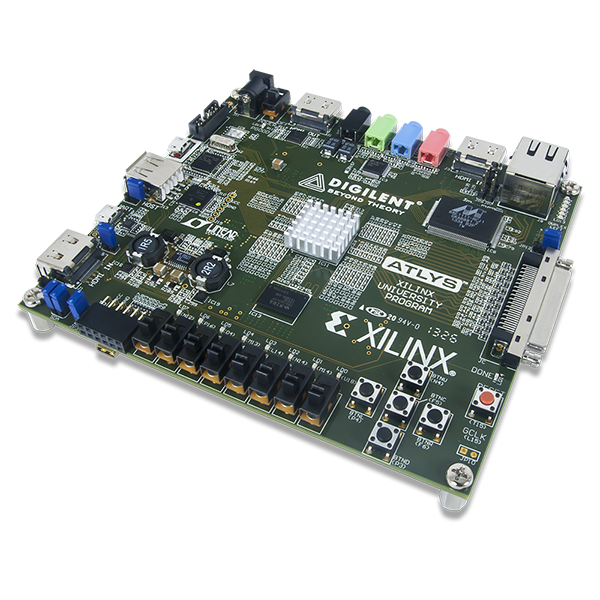
\includegraphics[width=8cm]{atlys_pic.png}
			\caption{Atlys Spartan-6 board}
		\end{subfigure}
		\hfill
		\begin{subfigure}[b]{.4\textwidth}
			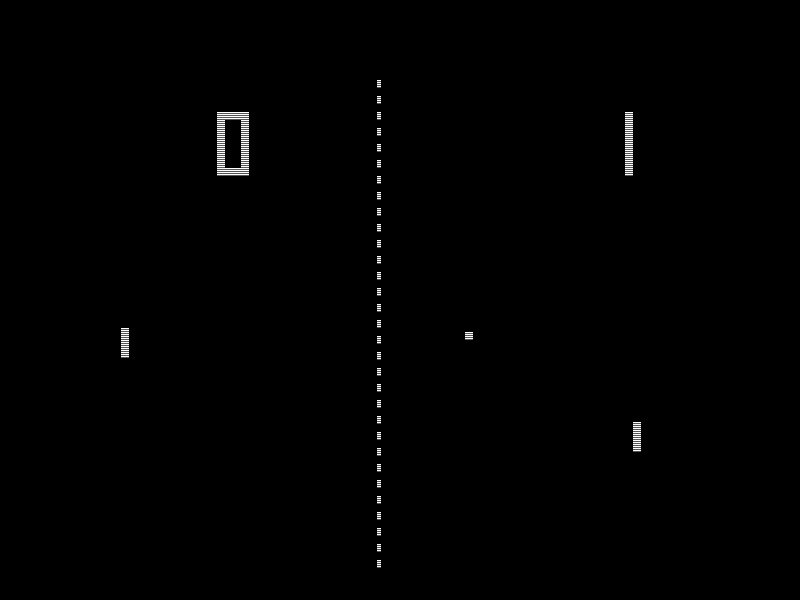
\includegraphics[width=8cm]{pong_screenshot.png}		
			\caption{Screenshot of the game Pong}
		\end{subfigure}
		
	\caption{Used board and screenshot of the game}
	\label{board+screenshot}
	\end{figure}
	
	
	\subsection{Block Diagram}
	\subsection{Functional Details}
	
\newpage
\section{Implementation}
	\subsection{Modules}
	\subsection{Results}
		\subsubsection{Synthesis and Implementation results}
	\subsection{Problems}

\newpage
\section{Assessment}

\newpage
\section{Summary}

\newpage
\section{Attachment}


\end{document}
